
%(BEGIN_QUESTION)
% Copyright 2006, Tony R. Kuphaldt, released under the Creative Commons Attribution License (v 1.0)
% This means you may do almost anything with this work of mine, so long as you give me proper credit

En enkel type elektronisk trykktransmitter kan bygges med et bourdon-rør og en \textit{differensiell kondensator}:

$$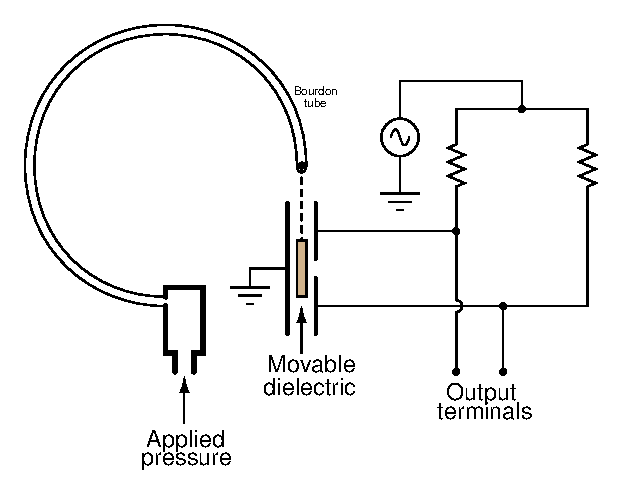
\includegraphics[width=15.5cm]{i00184x01.eps}$$

Forklar hvordan dette instrumentet virker, hvilken type elektrisk utgangssignal det genererer (f.eks. strøm, spenning, motstand osv.), og hvilken polaritet (om noen) utgangssignalet har.

\underbar{file i00184}
%(END_QUESTION)





%(BEGIN_ANSWER)

Hint: selv om det kanskje ikke ser slik ut ved første øyekast, danner de to motstandene en \textit{brokrets} sammen med den differensielle kondensatoren.

%(END_ANSWER)





%(BEGIN_NOTES)

Utgangen er en AC-spenning med amplitude proporsjonal med dielektrikums posisjon, som igjen er proporsjonal med pålagt trykk.

Denne instrumentutformingen er trolig lite praktisk med mindre utgangsdetektorkretsen plasseres svært nær brokomponentene, for å redusere parasittkapasitans.

\vskip 10pt

Det kan være nyttig å repetere denne formelen med studentene når kapasitansbasert instrumentering diskuteres:

$$C = {\epsilon A \over d}$$

\noindent
Hvor,

$C =$ Kapasitans i Farad

$\epsilon =$ Permittivitet i dielektrikum (absolutt)

$A =$ Lederareal, i kvadratmeter

$d =$ Avstand mellom lederne, i meter

%INDEX% Measurement, pressure: differential capacitor as bourdon tube sensor

%(END_NOTES)

